\chapter{Introduction to Reinforcement Learning}

The reinforcement learning (RL) method aims to make the sequential decision:

\section{Sequential Decision Problem}
\paragraph{Background}
Suppose $N>0$ is the \emph{time horizon} of the decision problem. 
The symbol $x_k\in\mathcal{X}_k$ refers to the \emph{state} at time $k$, for each $k\in[0,N+1]$. 
At time $k$, after obverving the state $x_k$, we are required to take an appropriate action $a_k\in\mathcal{A}_k$. 
Given $(x_k,a_k)$, a new (\emph{random}) state $x_{k+1}$ is observed and a \emph{one-step} (\emph{stage}) cost $g_k(x_k,a_k,x_{k+1})$ is incurred.
The sequence $(x_0,a_0,x_1,a_1,\dots,x_N,a_N,x_{N+1})$ is known as an \emph{episode}.
\paragraph{Objective}
The goal is to minimize the expected total cost:
\begin{enumerate}
\item
The total cost for one given episode is
\begin{equation}
\sum_{k=0}^Ng_k(x_k,a_k,x_{k+1})
\end{equation}
\item
Here $\pi=\{\mu_0,\dots,\mu_N\}$ is called a policy, with a collection of functions 
\begin{equation}
\begin{array}{ll}
\mu_k:\mathcal{X}_k\to\mathcal{A}_k,
&
a_k=\mu_k(x_k)
\end{array}
\end{equation}
\item
The expected total cost under total cost $\pi$ is given by:
\begin{equation}
J_{\pi}(x)=\mathbb{E}_{\pi}\left[
\sum_{k=0}^Ng_k(x_k,a_k,x_{k+1})\middle| x_0=x
\right]
\end{equation}
where $\mathbb{E}_{\pi}$ is the expectation over randomness for transitions from $x_k$ to $x_{k+1}$, $k\in[0,N]$, under the policy $\pi$.
\item
Therefore, we aim to solve the policy-based optimization problem given the initial state $x$:
\begin{equation}
J^*(x)=\inf_{\pi}J_{\pi}(x)
\end{equation}
\end{enumerate}
We say a policy $\pi^*$ is an \emph{optimal policy} if $J^*(x)=J_{\pi^*}(x)$. However, the infimum may not be achievable, i.e., the optimal poplicy may not exist. In our setting, we only focus on the case where the optimal policy can be achieved.



\paragraph{Possible Types of Dynamics}
The transition from $x_k,a_k$ to $x_{k+1}$ can be modelled by the transition probability:
\[
\begin{array}{ll}
\mathbb{P}\left\{
x_{k+1}=y\middle|x_k=x,a_k=a
\right\}
=
P_k(x,a,y),
&
\forall x\in\mathcal{X}_k,a_k\in\mathcal{A}_k,y\in\mathcal{X}_{k+1}.
\end{array}
\]
We will possibly face three different cases for this problem
\begin{enumerate}
\item
When the transition probabilities are known, this is the so-called \emph{perfect information} case. This problem reduces to the \emph{markov decision problem}, which can be solved by applying \emph{dynamic programming}
\item
When the transition probabilities are unknown, but we can get many epsiodes from data. In this case, we can estimate the transition probability, but the computation cost is expansive.
\item
When the transition probabilities are unknown, but given $(x_k,a_k)$, we can sample for $x_{k_1}$, i.e., \emph{a simulator is available}. This case is between case 1 and 2, and the corresponding solution will be talked later.
\end{enumerate}

\paragraph{Solving for Case (1)}
\begin{itemize}
\item
When $N$ is finite, We set the cost-to-go function $J_k$ to be the total cost starting from the $k$-th stage into the final state:
\begin{align*}
J_{N+1}&=0,\qquad x\in\mathcal{X}_{N+1}, \ \text{and for }k=N,N-1,\dots,0,\\
J_k(x)&=\min_{a\in\mathcal{A}_k(x)}\mathbb{E}_{P_k(x,a,y)}\left[g_k(x,a,y)+J_{k+1}(y)\right],\quad x\in\mathcal{X}_k\\
&=\min_{a\in\mathcal{A}_k(x)}\sum_{y\in\mathcal{X}_{k+1}}
P_k(x,a,y)
\left[
g_k(x,a,y)+J_{k+1}(y)
\right]\\
J^*(x)&=J_0(x),\quad x\in\mathcal{X}_0
\end{align*}
This is so-called \emph{backward induction algorithm}. The drawback is due to its huge complexity. To obtain the optimal solution, when $N$ is large, we need $\prod_{k=0}^N|\mathcal{A}_k||\mathcal{X}_{k+1}|$ computation times, though in some special problem this complexity can be reduced.
\item
When $N$ is infinite, the problem becomes easier to solve suprisingly. Assume the time homogeneity with a discounted factor $\beta<1$, i.e., the transition probability $P_k$ remains the same for large $k$, and the stage cost gradually decreases with discounted factor $\beta$ and underlying cost function $g$:
\[
\begin{array}{ll}
P_k=P,
&
g_k=\beta^kg
\end{array}
\]
As a result, it suffices to solve the \emph{Bellman equation}:
\begin{equation}
J^*(x)=\min_{a\in\mathcal{A}}\sum_{y\in\mathcal{X}}P(x,a,y)\left(
g(x,a,y)+\beta J^*(y)
\right)
\end{equation}
\end{itemize}
Let's discuss the Bellman equation in detail.

\section{Bellman's Equation}
Here the key assumption follows from the last section: Assume the time homogeneity with a discounted factor $\beta<1$.
\paragraph{Notation}
We use the notation $P(x,a,y)$ to denote the conditional probability $\mathbb{P}\{x'=y\mid x,a\}$ for $y\in\mathcal{X}$, and write the summation over probabilties in an expectation form:
\[
\sum_{x'\sim P(\cdot\mid x,a)}
\left[
g(x,a,x')+\beta J^*(x')
\right]
\]

Actually, Bellaman~[\cite{ber1995}] tells us that we can find the solution from the Bellaman equation:
\begin{theorem}
Assume that the state space $\mathcal{X}$ and action space $\mathcal{A}$ is finite.
The optimal value function $J^*$ is the \emph{one and only one} solution solution to the Bellman's equation:
\begin{equation}
J^*(x)=\min_{a\in\mathcal{A}}
\mathbb{E}_{x'\sim P(\cdot\mid x,a)}
\left(
g(x,a,x')+\beta J^*(x')
\right)
\end{equation}
\end{theorem}

After obtaining the optimal solution $J^*$, we can derive a policy $J^*$, which is one of the optimal policy to our decision problem:
\begin{theorem}
Assume that the state space $\mathcal{X}$ and action space $\mathcal{A}$ is finite.
Let $J^*:\mathcal{X}\to\mathbb{R}$ be the unique solution to the Bellman equation.
Define $\mu^*:\mathcal{X}\to\mathcal{A}$ via
\[
\mu^*(x)=\arg\min_{a\in\mathcal{A}(x)}\mathbb{E}_{x'\sim P(\cdot\mid x,a)}
\left(
g(x,a,x')+\beta J^*(x')
\right),\qquad
\forall x\in\mathcal{X}
\]
\end{theorem}

\paragraph{Notation}
\begin{itemize}
\item
For a function $h\in\mathcal{X}\to\mathbb{R}$, define the \emph{$h$-greedy policy} $\mu_h:\mathcal{X}\to\mathcal{A}$ via
\[
\mu_h(x)=\arg\min_{a\in\mathcal{A}(x)}\mathbb{E}_{x'\sim P(\cdot\mid x,a)}
\left(
g(x,a,x')+\beta h(x')
\right),\qquad
\forall x\in\mathcal{X}
\]
Here you may understand $h$ as the tradeoff for minimizing between the current cost $g$ and the future cost, and therefore $J^*$-greedy policy tells us how to make optimal policy for the given decision problem.
\item
Also define the \emph{Bellman operator} $T$ for $J$: $\mathcal{X}\to\mathbb{R}$, with
\begin{equation}
(TJ)(x) = \min_{a\in\mathcal{A}(x)}\mathbb{E}_{x'\sim P(\cdot\mid x,a)}
\left(
g(x,a,x')+\beta J(x')
\right)
\end{equation}
\item
Fix a stationary policy $\mu$, we assume that $\mu(x)$ admits only one value (randomly choose one value from $\mu(x)$ is also ok), and therefore define the Bellman operator for $J$ w.r.t. $\mu$: $\mathcal{X}\to\mathbb{R}$, with
\begin{equation}
(T_\mu J)(x) = \mathbb{E}_{x'\sim P(\cdot\mid x,a)}
\left(
g(x,\mu(x),x')+\beta J(x')
\right)
\end{equation}
\item
Therefore for any $J$, 
\begin{equation}
(T_{\mu_J}J)(x)=(TJ)(x),\ \forall x\in\mathcal{X}
\end{equation}
\end{itemize}

\paragraph{Method for solving Bellman equation: value iteration}
Starting with arbitrary $J^0:=J$, we define the value iteration function $J^n=TJ^{n-1}$. The \emph{value iteration} guarantees to converge finally: 
\begin{theorem}
For any function $J:\mathcal{X}\to\mathbb{R}$, we have for all $x\in\mathcal{X}$:
\[
J^*(x)=\lim_{N\to\infty}(T^NJ)(x).
\]
\end{theorem}
The convergence rate is easy to show:
\begin{align*}
\max_{x\in\mathcal{X}}|J^N(x)-J^*(x)| & =\max_{x\in\mathcal{X}}|TJ^{N-1}(x)-TJ^*(x)|\\
&\le \beta\max_{x\in\mathcal{X}}|J^{N-1}(x)-J^*(x)|\\&\le \beta^N\max_{x\in\mathcal{X}}|J(x)-J^*(x)|.
\end{align*}
Therefore, we have two alternatives to guarantee fast convergence rate. One is to find a small discount factor; another way is to make good initial guess for $J^0$. 

%\subsection{Complexity Analysis}

\paragraph{Complexity Analysis for value evaluation}
The calculation for $J^n(x)=(TJ^{n-1})(x)$ requires the complexity $|\mathcal{A}||\mathcal{X}|$:
\[
J^n(x)=\min_{a\in\mathcal{A}(x)}\left[
g(x,a)+\beta\sum_{x\in\mathcal{X}}P(x,a,y)J^{n-1}(y)
\right]
\]
Therefore the complexity for $N$ steps is $N\cdot |\mathcal{A}|\cdot |\mathcal{X}|^2$.

\subsection{Searching for optimal policy}
\paragraph{Criteria for the performance of policy}
Given a stationary policy $\mu$, assume that the \emph{value function} $J_\mu$ satisfies the Bellman equation
\begin{equation}\label{Eq:1:10}
J_\mu(x)=g(x,\mu(x))+\beta\sum_{y\in\mathcal{X}}P(x,\mu(x),y)J_\mu(y),\ \quad x\in\mathcal{X}
\end{equation}
Therefore, the expected cost w.r.t. $\mu$ is given by:
\begin{equation}\label{Eq:1:11}
J_\mu = (I-\beta P_\mu)^{-1}g_\mu,
\end{equation}
where $g_\mu$ is an $|\mathcal{X}|$-vector with entries $g_\mu(x) = g_\mu(x,\mu(x))$; $P_\mu$ is an $|\mathcal{X}|\times|\mathcal{X}|$ matrix with entries $P_\mu(x,y)=P(x,\mu(x),y)$.

The complexity of (\ref{Eq:1:11}) is huge, but there are many other algorithms for solving (or approximately solving) (\ref{Eq:1:10}).

\paragraph{Algorithm for searching for optimal policy}
The basic algorithm for deriving an optimal (stationary) policy is listed as follows:
\begin{enumerate}
\item
Initialization: guess an initial stationary policy $\mu^0$.
\item
Policy evaluation: find $J_{\mu^k}$
\item
Policy Improvement: Obtain a new stationary policy $\mu^{k+1}$ that is $J_{\mu^k}$-greedy
\item
Stop Criteria: if $J_{\mu^k}=J_{\mu^{k+1}}$, then stop, otherwise go to step 2.
\end{enumerate}
\begin{figure}[H]
\centering
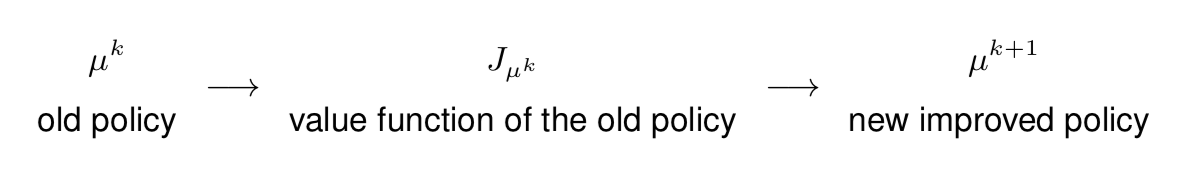
\includegraphics[width=1\textwidth]{First_lecture/p_1}
\caption{Diagram for the algorithm above}
\end{figure}
\paragraph{Convergence Issue}
Bellman gives the convergence of the algorithm, given the condition that the value function can be \emph{exactly evaluated}:
\begin{theorem}
Fix a policy $\mu$. Let $\hat{\mu}$ be a $J_\mu$-greedy policy, then we have
\[
J_{\hat \mu}(x)\le J_\mu(x),\ \text{for each }x\in\mathcal{X}.
\]
Moreover, if $\mu$ is not optimal, strict inequality holds for at least one state.
\end{theorem}
\begin{remark}
This theorem gives the convergence of the algorithm to the optimal policy. However, once we use algorithms to find the approximated value function due to the pity of hugh complexity for obtaining exact value function, the convergence to the optimal policy is no longer guaranteed
\end{remark}
\section{Reinforcement Programming}

\begin{itemize}
\item
The dynamic programming aims to solve the decision problem with the case where the \emph{model of the environment's dynamics is given ($P,g$ are known).}
\item
The reinforcement programming aims to solve the decision problem with the case where the \emph{model of the environment's dynamics is not given ($P,g$ are unknown), but the samples are available.}
\end{itemize}

Let's now focus on reinforcement learning only. First let's discuss issues about policy evaluation:
\subsection{Policy Evaluation}
Given a stationary policy $\mu$, the definition for value function $J_\mu(x)$ is given by:
\[
J_\mu(x)=\mathbb{E}\left[
\sum_{k=0}^\infty\beta^kg(x_k,\mu(x_k),x_{k+1})\middle|x_0=x
\right]
\]

To simplify the computation complexity, we find that the $J_\mu$ has to satisfy the one-step Bellman equation:
\begin{align*}
J_\mu(x)&=(T_\mu J_\mu)(x)\\
&=g_\mu(x)+\beta(P_\mu J_\mu)(x)\\
&=\mathbb{E}\left[g(x,\mu(x),x_1)\right]
+
\beta\mathbb{E}[J_\mu(x_1)]
\end{align*}

To get the approximated value function, we can equivalently solve
\begin{equation}\label{Eq:1:12}
J_\mu=\arg\min_{J\in\mathbb{R}^{|\mathcal{X}|}}\sum_{x\in\mathcal{X}}|J(x)-(T_\mu J)(x)|^2\xi(x)
\end{equation}
where the weight $\xi$ could be anything \emph{if (\ref{Eq:1:12}) is solvable}.

\paragraph{Bellman Error}
Therefore, there is a popular way to define the quality of the approximated value function:
\begin{equation}\label{Eq:1:13}
\|J-T_\mu J\|_{\xi}^2\equiv \sum_{x\in\mathcal{X}}|J(x)-(g_\mu(x)+\beta(P_\mu J)(x))|^2\xi(x)
\end{equation}
where $\xi$ is commonly chosen as the stationary distribution of the DTMC with transition matrix $P_\mu$, i.e., more visited states should be weighted more. Note that the $\xi$ may not be explicitly derived, but only for simplicity of analysis.

\paragraph{Optimization for the loss function~(\ref{Eq:1:13})}
By taking gradient of (\ref{Eq:1:13}) wr.t. $J$ to $0$, we obtain:
\begin{equation}\label{Eq:1:14}
D(J - (g_\mu+\beta P_\mu J))=0,
\end{equation}
where $D$ is the diagonal matrix with $\xi$ along the diagonal.
Note that (\ref{Eq:1:14}) is equivalent to solving the fixed point problem
\begin{equation}
J = J - \gamma \underbrace{D[(I-\beta P_\mu) J - g_\mu]}_{(*)},
\end{equation}
where the term (*) can be expressed as
\begin{equation}\label{Eq:1:16}
D[(I-\beta P_\mu) J - g_\mu] = \mathbb{E}_\xi\left[J(x) - \beta J(x') - g(x,x')\right]
\end{equation}

\paragraph{Tabular TD(0) Learning}
The Equations (\ref{Eq:1:13})-(\ref{Eq:1:16}) motivates the TD learning below:
\begin{enumerate}
\item
(Initialization) Initialize $J^0$, choose initial state $x_0$.
\item
(Simulation) simulate one step (once) staring from $x_k$, with the decision given by $\mu$. Our observation is the next state $x_{k+1}$ and the one-step cost $g_k$
\item
(Update) Our update is as follows:
\begin{equation}
\left\{
\begin{aligned}
J^{k+1}(x_k)&=J^k(x_k) - \gamma_k\left[ J^k(x_k) -  (g_k + \beta J^k(x_{k+1}))\right],\\
J^{k+1}(y) &= J^k(y), \ \text{for }y\ne x_k
\end{aligned}
\right.
\end{equation}
\item
Set $k=k+1$ and go to step 2.
\end{enumerate}
\begin{remark}
This algorithm only reuqires the update of parameters locally. The drawback for many other algorithms is that they require the global update for parameters, which is computationally difficult.
\end{remark}

The literature [\cite{Sutton1988}] gives the convergence analysis for this algorithm:
\begin{theorem}
Asume a Markov chain associated with the policy $\mu$ is \emph{finite, irreducible, and aperiodic}.
Given bounded costs $|g(x,a,x')|<G$ and learning rate such that, $\sum_{k=0}^\infty\gamma_k=\infty,\sum_{k=0}^\infty\gamma_k^2<\infty$, we have
\[
\lim_{k\to\infty}J^k=J_\mu \ \text{a.s.}
\]
\end{theorem}
\begin{remark}
One can have a similar algorithm but without focusing on one-step Bellman equation but $\ell$-step:
\[
J_\mu(x)=\mathbb{E}\left[\sum_{k=0}^\infty\beta^k g(x_k,\mu(x),x_{k+1})+\beta^{\ell+1}J_\mu(x_{\ell+1})\right]
\]
where $\ell\sim\text{Geometric}(\lambda)$ for $0\le\lambda\le1$. The corresponding algorithm is $\text{TD}(\lambda)$ learning algorithm, which will be discussed in the next lecture.
\end{remark}

\subsection{Policy Improvement}
Then we turn into the policy improvement. 
\paragraph{$Q$-Learning}
Approximation for $J_\mu$-greedy function requires defining an optimal $Q$-factor:
\begin{equation}\label{Eq:1:18}
\begin{aligned}
Q^*(x,a)&=\sum_{x'\in\mathcal{X}}P(x,a,x')\left[g(x,a,x')+\beta J^*(x')\right]\\
&=\mathbb{E}[g(x,a,x')+\beta J^*(x')]\\
&\approx\frac{1}{K}\sum_{i=1}^K\left(g(x,a,x_i')+\beta J^*(x_i')\right)
\end{aligned}
\end{equation}
Note that the argument for optimal $Q$-factor is a \emph{state-action} pair, which give an estimation of the performance for our action $a$. Therefore, the optimal policy is defined as
\begin{equation}\label{Eq:1:19}
\mu^*(x)=\arg\min_{a\in\mathcal{A}(x)}Q^*(x,a)
\end{equation}
\begin{remark}
When $Q^*$ is too big or solving (\ref{Eq:1:19}) is too difficult, we need a low dimensional representation of $Q^*$.
\end{remark}

\paragraph{Bellman equation for $Q$-factor}
The definition~(\ref{Eq:1:18}) motivates to define a way to compute $Q$-factor by the Bellman equation. First define
\begin{equation}
(TQ)(x,a)=\sum_{y\in\mathcal{X}}P(x,a,y)\left[g(x,a,y)+\beta\min_{v\in\mathcal{A}(y)}Q(y,v)\right]
\end{equation}
Then $Q^*$ is the unique fixed point to the equation $Q=TQ$.
\begin{remark}
When both $P$ and $g$ are known, the value iteration $Q_{k+1}=TQ_k$ converges to $Q^*$ from any staring $Q_0$; otherwise we need to sample to approximate $P$, and therefore the convergence may not be guaranteed.

Also, the policy obtained in each iteration is a deterministic value, and therefore we can introduce a stochastic policy evaluation algorithm.
\end{remark}

\paragraph{$Q$-Learning as a stochastic version}
\begin{enumerate}
\item
First generate long sequence of $\{x_k,a_k,g_k\}$ s.t. the state-action pair $(x,a)$ appears infinitely often.
\item
Then the $Q$-factor of $(x_k,a_k)$ pair is updated:
\begin{equation}
\left\{
\begin{aligned}
Q_{k+1}(x_k,a_k)&=(1-\gamma_k)Q_k(x_k,a_k)+\gamma_k\left(g_k+\beta\min_vQ_k(x_{k+1}',v)\right)\\
Q_{k+1}(x,a)&=Q_k(x,a),\ \text{if }(x,a)\ne(x_k,a_k)
\end{aligned}
\right.
\end{equation}
\item
Note that $g_k+\beta\min_vQ_k(x_{k+1}',v)$ is a single sample approximation of the expected value $(TQ)(x_k,a_k)$.
\end{enumerate}


The literature [\cite{Watkins92}] gives a convergence result for the $Q$-learning:
\begin{theorem}
Given the condition that:
\begin{enumerate}
\item
A sequence where each state-action pair appears \emph{infinitely often}
\item
The stage cost is bounded, i.e., $|g(x,a,y)|<G$
\item
The learning rate $\gamma_k\in(0,1)$ is such that $\sum_{k=0}^\infty\gamma_k=\infty,\sum_{k=0}^\infty \gamma_k^2<\infty$
\end{enumerate}
The $Q$-learning algorithm converges:
\[
\lim_{k\to\infty}Q_k(x,a)=Q^*, \ \text{a.s.}
\]
\end{theorem}
\begin{remark}
The theory of reinforcement learning requires ambitious condition, and in practice we can only make the approximation. Therefore, most of algorithms are heuristic. 
\end{remark}

\subsection{Policy Iteration using $Q$-factors}
\begin{itemize}
\item
(Policy Evaluation):
Given current policy $\mu^k$, we find the fixed point $Q_{\mu^k}$ for the equation
\[
Q(x,a)=\sum_{y\in\mathcal{X}}P(x,a,y)[g(x,a,y)+\beta Q(y,\mu^k(y))]
\]
\item
(Policy Improvement): 
Find $\mu^{k+1}(x)$ based on $Q_{\mu^k}$:
\[
\mu^{k+1}(x)=\arg\min_{a\in\mathcal{A}(x)}Q_{\mu^k}(x,a)
\]
\end{itemize}

Here the question turns out that how to make the policy evaluation regarding $Q$:

\paragraph{SARSA Heuristic Algorithm}
\begin{enumerate}
\item
(Initialization): arbitrary initialize $Q^0$, choose initial state $x_0$, initial decision $a_0$
\item
(Simulation): simulate one step starting from $x_k$, with the decision given by $a_k$. Observe the next state $x_{k+1}$ and the cost $g_k$
\item
(Evaluation $\&$ Improvement):
\[
a_{k+1}
=
\left\{
\begin{aligned}
\arg\min_{a\in\mathcal{A}}Q^k(x_{k+1},a),&\quad \text{w.p. }1-\varepsilon\\
\text{other action},&\quad \text{w.p. }\varepsilon
\end{aligned}
\right.
\]
\item
(Update):
\[
\left\{
\begin{aligned}
Q^{k+1}(x_k,a_k)&=(1-\gamma_k)Q^k(x_k,a_k)+\gamma_k\left[g_k+\beta Q^k(x_{k+1},a_{k+1})\right],\\
Q^{k+1}(y,v)&=Q^k(y,v),\quad \text{for }(y,v)\ne(x_k,a_k)
\end{aligned}
\right.
\]
\item
$k=k+1$, move into step 2.
\end{enumerate}
\[
SARSA: \text{State}\to\text{Action}\to\text{Reward}\to\text{State}\to\text{Action}
\]













%\bibliographystyle{IEEEtran}
%\bibliography{paper.bib}







